\documentclass[12pt,dvipdfmx]{jarticle}
%\documentstyle[12pt,fleqn,epsf,iepaper,cite]{jarticle}
%\documentstyle[12pt,iepaper,eclepsf,oddchar]{jarticle}

\usepackage{colortbl}
\usepackage{multicol}
\usepackage{amsmath}
\usepackage{amssymb}
\usepackage{amsfonts}
\usepackage{mathbbol}
\newcommand{\bm}[1]{{\mbox{\boldmath $#1$}}}
\usepackage{cite}


\usepackage[dvipdfm]{graphicx}
\usepackage{iepaper}
\usepackage{epsf}
\usepackage{ccaption}
\usepackage{pdfpages}

\title{遺伝的アルゴリズムによる機械学習における\\疑似ラベル生成手法の提案}
\author{細川 岳大}
\gakuseki{1171201161}[B]  %卒論はB,修論はM
\group{第 1 研究グループ}            % 卒論の場合
\shidou{森 直樹 教授}                          % 卒論の場合
%\syusa{教授}                            % 修論の場合
%\hukusa{教授}{教授}

%図番号を「(section番号).(図番号)」とするため
\makeatletter
\renewcommand{\thefigure}{%
	\thesection.\arabic{figure}}
\@addtoreset{figure}{section}
\makeatother
\makeatletter
\renewcommand{\thetable}{%
	\thesection.\arabic{table}}
\@addtoreset{table}{section}
\makeatother
\makeatletter
\renewcommand{\theequation}{%
	\thesection.\arabic{equation}}
\@addtoreset{equation}{section}
\makeatother


\begin{document}
	\maketitle
	
	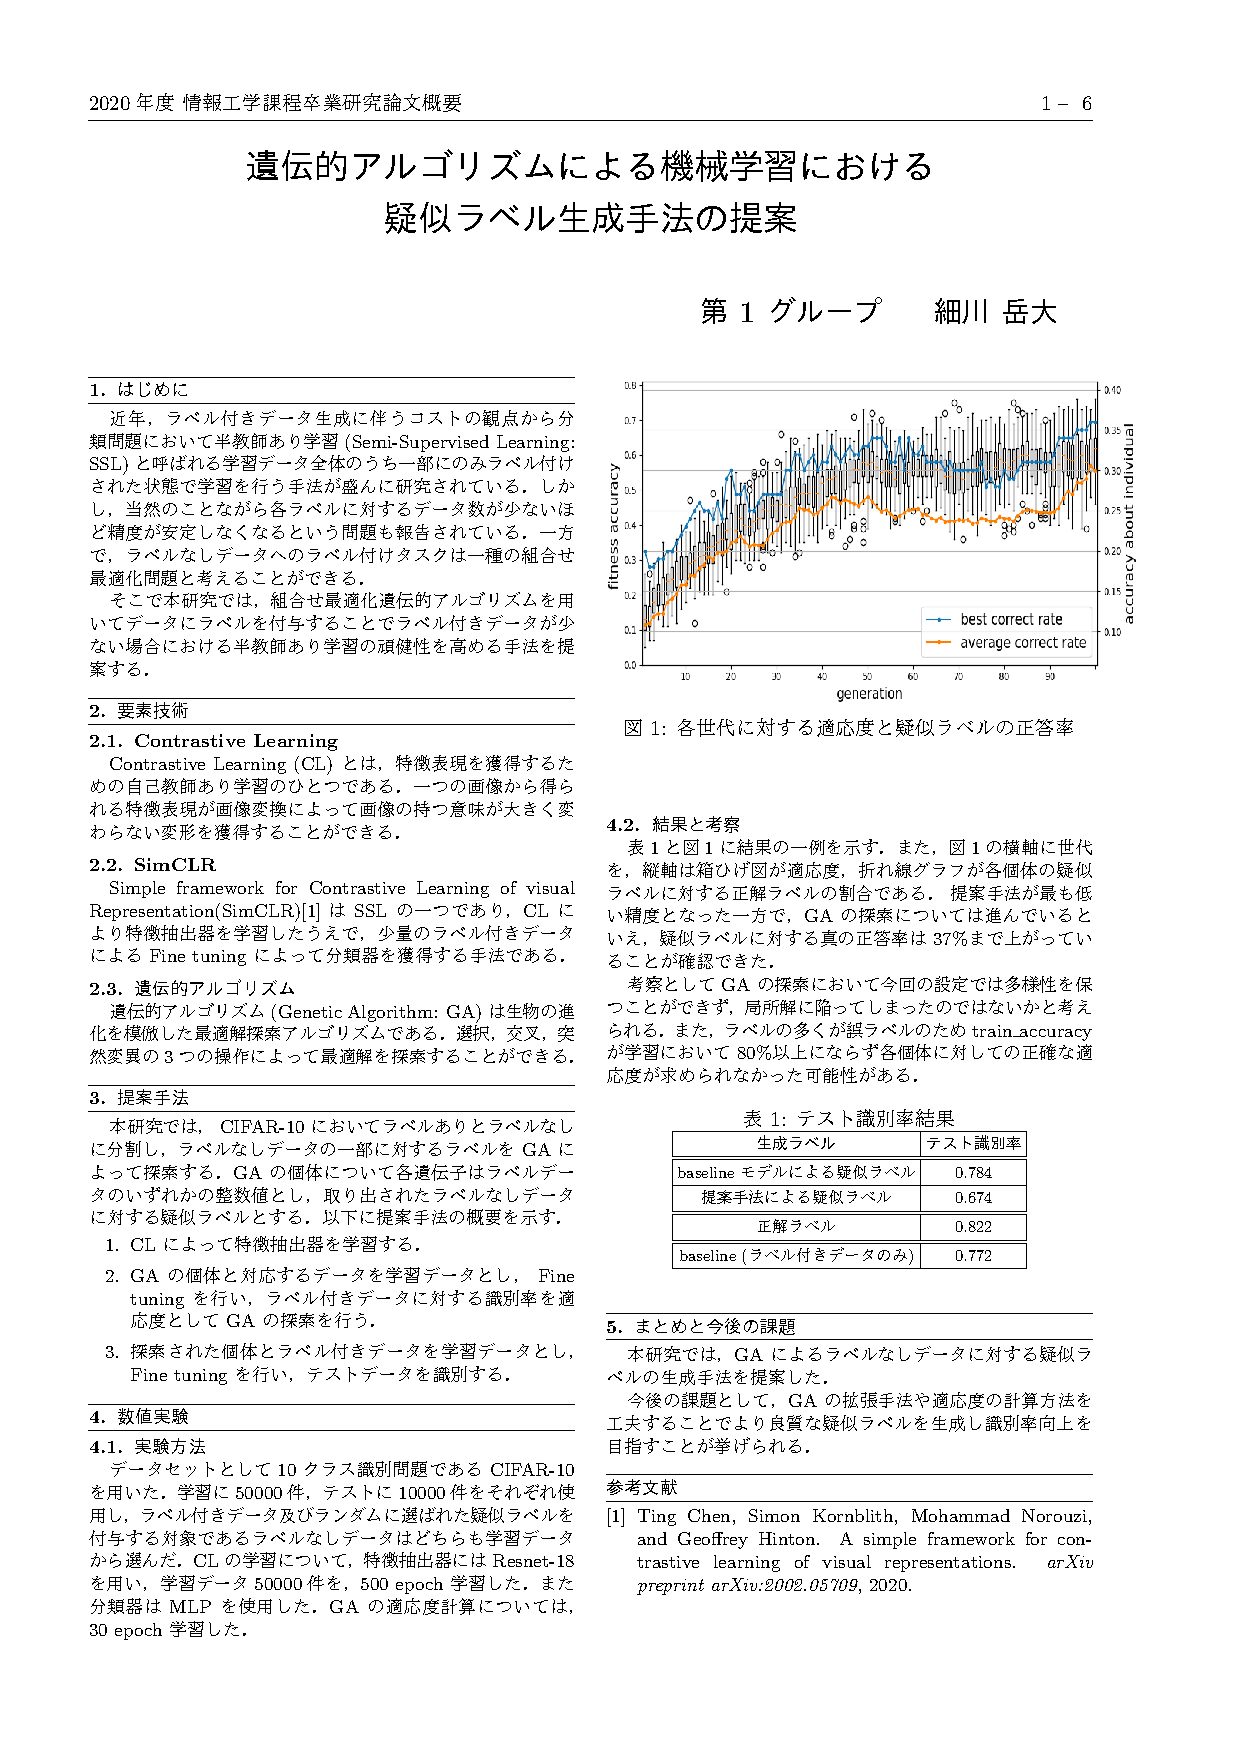
\includepdf[fitpaper]
	{../abstract/abstract_2020_final_hosokawa.pdf}
	\pagenumbering{roman}
	%%% 目次
	\tableofcontents
	\newpage
	%
	%% 図一覧
	\listoffigures
	\newpage
	
	%% 表一覧
	\listoftables
	\newpage
	
	\pagenumbering{arabic}
	
	% 文書開始
	\newpage
\changeindent{0cm}
\section{はじめに}
\changeindent{2cm}
近年,機械学習の発展に伴い,様々な分野への応用がされており
様々な新規データセットにおいて目覚ましい結果が報告されている.
また新規データセットを生成する際,分類問題では各データにふさわしいラベル付けをする必要があるが,
ラベル付けには人の手が必要でありコストがかかる問題がある.
そこで半教師あり学習 (Semi-Supervised Learning: SSL)と呼ばれる
学習データ全体のうち一部にのみラベルが付与された状態で学習を行う手法が提案されており,
盛んに研究されている.また最新の SSL の手法では,全データにラベルが付与されている教師あり学習にも劣らない成果の報告\cite{sohn2020fixmatch}もある.しかし,当然のことながら各ラベルに対するデータ数が少ないほど精度が安定しなくなるという報告もされている.

一方,ラベルなしデータへのラベル付けタスクは一種の組合せ最適化問題と考えることができる.

本研究では,組合せ最適化問題に有効である遺伝的アルゴリズムを用いてデータにラベルを付与することでラベル付きデータが少ない場合における半教師あり学習の頑健
性を高める手法を提案する.

以下に本論文の構成を示す.まず,2章では本研究で用いる要素技術につ
いて概説する.続いて3章で実験手法の提案をし,4章において実験結果と考察を
示す.5章で本研究の成果をまとめたうえで,今後の課題について述べる.


	\clearpage
	%要素技術
	\newpage
\changeindent{0cm}
\section{要素技術}
\changeindent{2cm}

本章では,実験に関連する要素技術について説明する.

\changeindent{0cm}
\subsection{半教師あり学習}
\changeindent{2cm}
半教師あり学習 (Semi Supervised Learning: SSL)\cite{zhu2005semi,chapelle2009semi} は
大量のラベルなしデータと少量のラベル付きデータを用いて学習を行う手法である.


\changeindent{0cm}
\subsection{疑似ラベル}
\changeindent{2cm}
疑似ラベル (Pseudo Label)\cite{lee2013pseudo} はあるモデルによって予測されるラベルなしデータに対する暫定的なラベルである.
 SSL では疑似ラベルを付与したデータをラベル付きデータに混ぜて学習することで各ラベル同士に対する確率分布を粗密なものにする作用があり,正則化\cite{grandvalet2006entropy}の役割をする.データ数を $N$\ ,あるモデルによる予測確率を $q_b$\ ,予測確率 $p, q$\ に対する Cross Entropy Loss を ${\rm H}(p,q)$\ ,閾値を $\tau$ とするとき,(\ref{quadPL})式で与えられる.
 
 \begin{equation}
 \hat{q}_b = {\rm argmax}(q_b)
 \end{equation}
 \begin{equation}
 \label{quadPL}
 \frac{1}{N}\sum^{N}_{b=1}
 {\mathbb{1}({\rm max}(q_b)\geq\tau){\rm H}(\hat{q}_b,q_b)}
 \end{equation}
 
\changeindent{0cm}
\subsection{FixMatch}
\changeindent{2cm}
FixMatch\cite{sohn2020fixmatch}\ は\ SSL\ の一つである.
図\ref{fig:FixMatch}に\ FixMatch\ の概略図を示す.
疑似ラベルと Consistency Regularization の二つの正則化手法を
統合させた手法である.


\begin{figure}[h]
	\begin{center}
		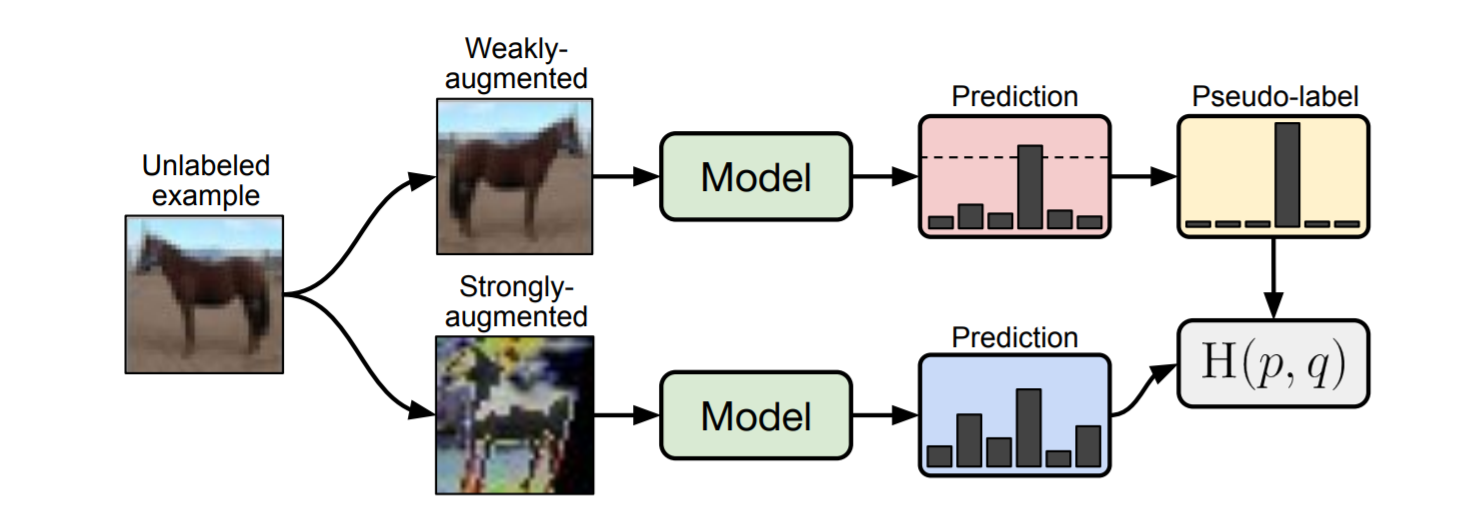
\includegraphics[scale=0.6]{./images/FixMatch.PNG}
		\caption[FixMatch の概略図]
		{FixMatch の概略図 (: 文献\cite{sohn2020fixmatch}の Figure 1 を参照\label{fig:FixMatch})}
	\end{center}
\end{figure}

\changeindent{0cm}
\subsubsection{RandAugment}
\changeindent{2cm}
RandAugment \cite{cubuk2020randaugment} とは,データ拡張手法の一つであり,
チューニングするパラメータは $N$ と $M$ の二種類で,複数あるデータ変換操作のうちランダムに $N$ 個選択し
変換強度 $M$ で順に適用する手法である.FixMatch では強変換として用いられる.


\changeindent{0cm}
\subsubsection{Consistency Regularization}
\changeindent{2cm}
Consistency Regularization \cite{zhang2019consistency} は正則化手法の一つであり,
画像による変換の前後で予測値が変わらないようなロスを与える.ラベルなしデータを$u_b$\ ,
 $\alpha(\cdot)$ を画像変換,$p_{\rm m}(y|x)$ を入力 $x$ に対するモデルの出力とすると,
(\ref{quadCR})式で与えられる.

\begin{equation}
\label{quadCR}
\sum^{N}_{b=1}{||p_{\rm m}(y|\alpha_1(u_b)) - p_{\rm m}(y|\alpha_2(u_b))||^2_2}
\end{equation}

\changeindent{0cm}
\subsubsection{更新}
\changeindent{2cm}
まず,バッチサイズを $B$ としラベル付きデータを ${\cal X} = {(x_b, p_b): b \in (1, ... ,B)}$ 
としたとき,ラベル付きデータに対するロスを ${\ell}_{\rm s}$ とすると,(\ref{quadLs})式で与えられる.

\begin{equation}
\label{quadLs}
{\ell}_{\rm s} = \frac{1}{B}\sum^{B}_{b=1}{\rm H}(p_b,p_{\rm m}(y|\alpha(x_b)))
\end{equation}

また,ラベルなしデータに対するロス ${\ell}_{\rm u}$ は,(\ref{quadPL}),(\ref{quadCR})式より,

\begin{equation}
\label{quadLu}
{\ell}_{\rm u} = \frac{1}{\mu B}\sum^{\mu B}_{b=1}
{\mathbb{1}({\rm max}(q_b)\geq\tau){\rm H}(\hat{q}_b,p_{\rm m}(y|{\cal A}(u_b)))}
\end{equation}

となる.このとき,$\mu$ はバッチ内のラベル付きデータに対するラベルなしデータの比率,$\cal A(\cdot)$は強変換である.

従って,ラベルなしデータの重みを$\lambda$	として,バッチ全体のロスは ${\ell}_{\rm s}+\lambda {\ell}_{\rm u}$ となる.

\changeindent{0cm}
\subsection{SimCLR}
\changeindent{2cm}
Simple framework for Contrastive Learning of visual Representation(SimCLR)\cite{chen2020simple}は SSL の一つである.
図\ref{fig:SimCLR}に概略図を示す.モデルの構造は Encoder,Projection Head,Classsifier
から構成されており, Encoder と Projection Head に対して,全データを用いて Contrastive Learning によって学習する.次に学習済みの Encoder と Classifier に対して,ラベル付きデータを用いて Classifier の学習を行う.最後にモデルの蒸留\cite{hinton2015distilling}を行うことで最終的なモデルを得る.

\begin{figure}[h]
	\begin{center}
		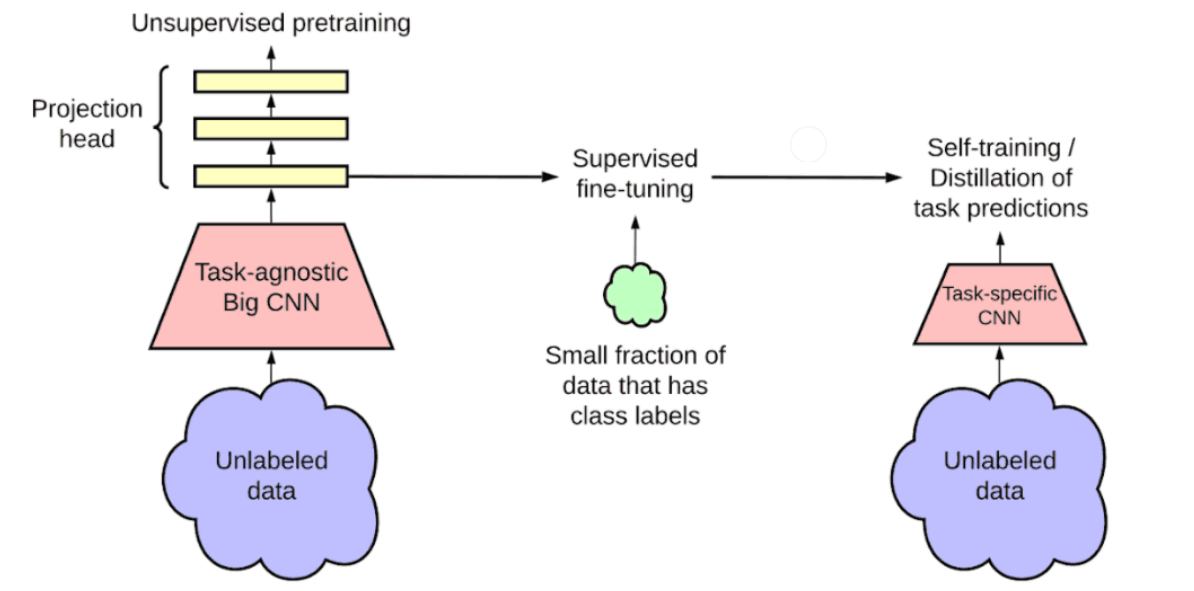
\includegraphics[scale=1.0]{./images/SimCLR.png}
		\caption[SimCLR の概略図]
		{SimCLR の概略図 (: 文献\cite{chen2020big}の Figure 3 を参照\label{fig:SimCLR})}
	\end{center}
\end{figure}

\changeindent{0cm}
\subsubsection{Cotrastive Learning}
\changeindent{2cm}
Contrastive Learning (CL)\cite{tian2020makes} とは特徴表現を獲得するための
自己教師あり学習\cite{doersch2017multi}のひとつである.
ある画像変換をした画像のペアについて元画像が一致するか否かを識別するタスクであり,
一つの画像から得られる特徴表現が画像変換によって
画像の持つ意味が大きく変化しないような Encoder を獲得することができる.
具体的な方法について,バッチ内の画像枚数を $N$ 枚とすると, Data Augmentation によって2倍に増やしたとき,
各画像に対して正例は1枚,負例は $2(N-1)$ 枚となる.このとき特徴ベクトル間の距離として cos 類似度を用いると,(\ref{sim})式で表される.また,正例との距離を小さくかつ,負例との距離を大きくするために正例のペア $({\bm z}_i,{\bm z}_j)$ に対するロス $\ell(i, j)$ は(\ref{quad_posl})式で表され,
バッチ全体のロス$\mathcal L$は(\ref{quad_L})式で表される.

\begin{equation}
\label{sim}
{\rm sim}({\bm u},{\bm v}) = {\bm u}^{\rm T}{\bm v}/\|{\bm u}\|\|{\bm v}\|
\end{equation}

\begin{equation}
\label{quad_posl}
\ell(i, j) = - {\rm log}\frac{{\rm exp}({\rm sim}({\bm z}_i, {\bm z}_j)/ \tau)}
{\sum_{k=1}^{2N}\mathbb{1}_{[k \neq i]}{\rm exp}({\rm sim}({\bm z}_i, {\bm z}_k)/ \tau)}
\end{equation}

\begin{equation}
\label{quad_L}
\mathcal L = \frac{1}{2N}\sum_{k=1}^{N}[\ell(2k-1,2k)+\ell(2k,2k-1)]
\end{equation}


\changeindent{0cm}
\subsection{ResNet}
\changeindent{2cm}
Residual Network (: ResNet)\cite{he2016deep} は Deep Neural Network (: DNN)\cite{larochelle2009exploring} のモデルの一つであり,
 DNNにおいて層を深くすることで発生する劣化問題及び勾配消失問題\cite{hochreiter1998vanishing}を解消するために残差についての学習を行うモデルである.図\ref{fig:ResBlock}に ResNet の構成要素である Residual Block の構造を示す.
2層の畳み込み層とショートカットを足し合わせた構造となっている.

\begin{figure}[h]
	\begin{center}
		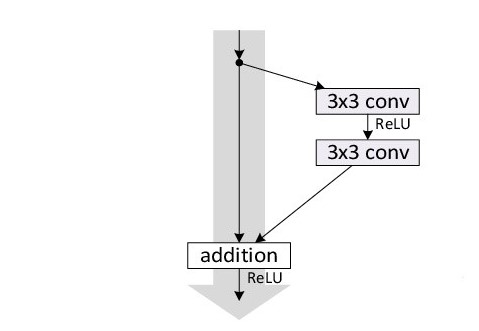
\includegraphics[scale=0.5]{./images/ResBlock.jpg}
		\caption[Residual Block の構造]
		{Residual Block の構造 (: 文献\cite{he2016identity}の Figure 2.(a) を参照\label{fig:ResBlock})}
	\end{center}
\end{figure}

\changeindent{0cm}
\subsection{Genetic Algorithm}
\changeindent{2cm}
遺伝的アルゴリズム (Genetic Algorithm: GA)\cite{whitley1994genetic} とは,生物の進化を模倣した組合せ最適化問題のアルゴリズムである.解の要素の最小単位を遺伝子,遺伝子の集まりである解を個体として表現する.また個体の集合を世代とし,各個体の計算された適応度をもとに選択,交叉,突然変異の3つの操作によって新たな個体群を生成し,次世代の個体集合とする.繰り返し世代を重ねることで最適解を探索する.
個体の基本的なエンコーディング方法として,バイナリ型,順列型,実数型,整数型がある.
本研究では整数型について扱うため,以下整数型を前提とした説明をする.

\changeindent{0cm}
\subsubsection{選択}
\changeindent{2cm}
選択\cite{blickle1996comparison}は自然淘汰をもとにした操作であり,個体の適応度にもとづき次世代に残される個体を選ぶものである.
以下のものがあげられる.
\begin{itemize}
	\setlength{\leftskip}{4.5cm}
	\item[エリート選択\cite{murata1996multi} : ]世代における適応度の最も高い個体を他の操作を行わず次世代に残す手法である.
	\item[トーナメント選択 : ]個体群からランダムに決められた数(: トーナメントサイズ)取り出し,
	その中で適応度の最も高い個体を選択する手法である.
\end{itemize}

\changeindent{0cm}
\subsubsection{交叉}
\changeindent{2cm}
交叉は生物の交配をもとにした操作であり,2つの個体から新たな2つの個体を生成するものである.
以下のものがあげられる.
\begin{itemize}
	\setlength{\leftskip}{3cm}
	\item[二点交叉 : ]対象となる2つの個体を同じ遺伝子座で3つに分割を行い,いずれかを入れ替える手法である.
	\item[一様交叉 : ]対象となる2つの個体についてある遺伝子座ごとにある確率で入れ替えを行う手法である.
\end{itemize}

\changeindent{0cm}
\subsubsection{突然変異}
\changeindent{2cm}
個体の遺伝子を変化させる操作で,局所探索になることを防ぐ.
乱数によって他の取りうる値に変化させる.また,突然変異率を上げすぎるとランダム探索となり,
収束しなくなるため,高くても数\%に設定されることが多い.


%CIFAR10\cite{krizhevsky2009learning}

%CL\cite{khosla2020supervised}
	\clearpage
	
	
\newpage
\changeindent{0cm}
\section{提案手法}
\changeindent{2cm}
本研究では,ラベルなしデータに対する疑似ラベルを GA を用いて
探索する手法を提案する.
また以降,半教師あり学習のデータについて学習データである
ラベル付きデータとラベルなしデータをそれぞれ $D_{\rm l}$\ ,$D_{\rm ul}$\ ,
テストデータを $D_{\rm t}$ と呼ぶ.


\changeindent{0cm}
\subsection{個体設定}
\changeindent{2cm}
まず,$D_{\rm ul}$からランダムにいくつかデータを取り出し探索データとする.
ここで,GAの扱う個体は探索データに対する疑似ラベル群である.
探索データと各遺伝子座は一対一対応しており,
遺伝子型は対応するラベルを表す整数値である.
従って,遺伝子長は探索データ数となる.
以降探索データについて $D_{\rm s}$ と呼ぶ.

\changeindent{0cm}
\section{提案手法}
\changeindent{2cm}
以下に提案手法の手順を示す.

\begin{enumerate}
	\item モデルの事前学習
	\item 事前学習したモデルに入力データを $D_{\rm s}$ ,ラベルデータを各個体とし
	学習し,$D_{\rm l}$ の識別率を適応度として GA の探索を行う.
	\item $D_{\rm l}$ と探索された個体をラベルとして持つ $D_{s}$ とを合わせてラベル付きデータとして
	 SSL によって再学習を行い $D_{\rm t}$ を識別する.
\end{enumerate}

既存の疑似ラベルを用いた手法では $D_{\rm s}$ で学習されるモデルの精度に大きく影響されるが,提案手法では疑似ラベルはモデルの出力ではないため正答率があがり,結果として半教師あり学習による精度も改善されることが期待できる.


	\clearpage
	
	\newpage
\changeindent{0cm}
\section{数値実験}
\changeindent{2cm}

本研究ではデータセットとして CIFAR-10\cite{krizhevsky2009learning} を用いた.
また実験1,2では半教師あり学習のベースモデルとしてそれぞれ FixMatch ,SimCLR を用いて GA によるラベル探索及び性能評価を行った.FixMatch と SimCLR で実験を行うことについて,同じ実験設定で同程度の精度を出すことができる一方
,FixMatch は毎回モデル全体を学習するのに対し SimCLR は出力層である分類器のみが学習される違いがある.

\changeindent{0cm}
\subsection{実験1}
\changeindent{2cm}

\changeindent{0cm}
\subsubsection{実験設定}
\changeindent{2cm}
表\ref{tb:ex1_data},\ref{tb:ex1_GApara},\ref{tb:ex1_FTXpara}にそれぞれ実験1における
各種設定を示す.また,FixMatch は学習に時間がかかるためラベル付きデータの一部を用いて事前学習をしたモデルの重みを初期重みとして使用する.

\begin{table}[h]
	\centering
	\caption{実験1 : データ内訳\label{tb:ex1_data}}
	\scalebox{1.0}{
		\begin{tabular}{|c||c|} \hline
			$D_{\rm l}$&250\\ \hline
			$D_{\rm ul}$&49650\\ \hline
			$D_{\rm s}$&100\\ \hline
			$D_{\rm t}$&10000\\ \hline
		\end{tabular}
	}
\end{table}


\begin{table}[h]
	\centering
	\caption{実験1 : GAの設定\label{tb:ex1_GApara}}
	\scalebox{1.0}{
		\begin{tabular}{|c|c|} \hline
			個体数&20\\ \hline
			世代数&20\\ \hline\hline
			選択&エリート + トーナメント\\ \hline
			エリート数&2\\ \hline
			トーナメントサイズ&2\\ \hline\hline
			交叉&二点交叉\\ \hline
			交叉率&1.0\\ \hline\hline
			突然変異&ランダム遷移\\ \hline
			遺伝子座ごとの突然変異率&0.02\\ \hline
		\end{tabular}
	}
\end{table}


\begin{table}[h]
	\centering
	\caption{実験1 : FixMatchの設定\label{tb:ex1_FTXpara}}
	\scalebox{1.0}{
		\begin{tabular}{|c|c|c|} \hline
			model&\multicolumn{2}{c|}{WideResNet16-2}\\ \hline\hline
			data set&\multicolumn{2}{c|}{cifar10}\\ \hline
			batch size&labeled&32\\ \cline{2-3}
			&unlabeled&$32*7$\\ \hline
			optimizer&\multicolumn{2}{c|}{SGD(lr=0.1,momntum=0.9)}\\ \hline
			loss&\multicolumn{2}{c|}{cross\_entropy\_loss}\\ \hline\hline
			\multicolumn{3}{|c|}{事前学習}\\ \hline
			train &labeled&100(:$D_{\rm l}$)\\ \cline{2-3}
			&unlabeled&49650(:$D_{\rm ul}$)\\ \hline			
			val data&\multicolumn{2}{c|}{150}\\ \hline
			num\_iterations&\multicolumn{2}{c|}{$2^{15}$}\\ \hline\hline
			\multicolumn{3}{|c|}{GAの評価}\\ \hline
			train &labeled&100(:$D_{\rm s}$)\\ \cline{2-3}
			&unlabeled&49650(:$D_{\rm ul}$)\\ \hline
			validation data&\multicolumn{2}{c|}{250(:$D_{\rm l}$)}\\ \hline
			num\_iterations&\multicolumn{2}{c|}{5000}\\ \hline\hline
			\multicolumn{3}{|c|}{探索された個体の評価}\\ \hline
			train &labeled&250(:$D_{\rm l}$)+$D_{\rm s}$\\ \cline{2-3}
			&unlabeled&49650(:$D_{\rm ul}$)\\ \hline	
			test data&\multicolumn{2}{c|}{10000(:$D_{\rm t}$)}\\ \hline
			num\_iterations&\multicolumn{2}{c|}{$2^{16}$}\\ \hline
		\end{tabular}
	}
\end{table}
\clearpage

\changeindent{0cm}
\subsubsection{結果と考察}
\changeindent{2cm}
図\ref{fig:ex1_res1},\ref{fig:ex1_res2}に GA の探索結果を示す.
図\ref{fig:ex1_res1}は横軸が GA の世代,縦軸は箱ひげ図が適応度,折れ線グラフは疑似ラベルの正答率で,図\ref{fig:ex1_res2}は横軸が疑似ラベルの正答率で縦軸が適応度を示している.
図\ref{fig:ex1_res2}から正の弱い相関性があることが確認できる一方で,図\ref{fig:ex1_res1}では
適応度のばらつきは減っており,学習自体は行われていることが確認できるものの疑似ラベルの正答率は全く向上していない.このことから,疑似ラベルの正答率と識別率は関係性があるが,誤ラベルの中に少量のラベル付きデータに対し過剰に適合するような局所解となりうるものの存在があると考えられる.

\begin{figure}[h]
	\begin{center}
		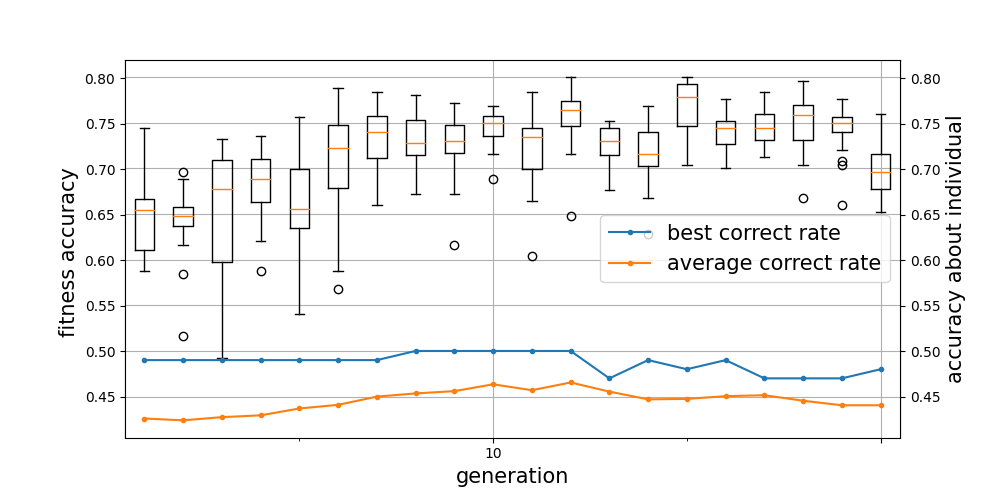
\includegraphics[scale=4.3]{./images/ex1_res_graph.png}
		\caption{実験1 : GA の探索結果\label{fig:ex1_res1}}
	\end{center}
\end{figure}
\clearpage

\begin{figure}[h]
	\begin{center}
		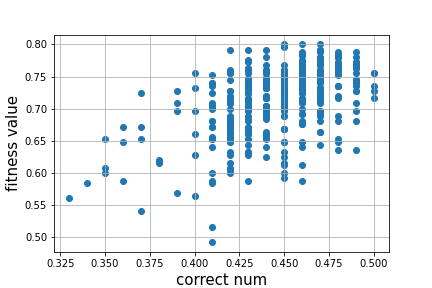
\includegraphics[scale=1.0]{./images/ex1_res_img.png}
		\caption{実験1 : 探索個体の散布図\label{fig:ex1_res2}}
	\end{center}
\end{figure}
\clearpage

次に,表\ref{tb:ex1_res3}に探索された個体によるテスト識別率を示す.
図\ref{fig:ex1_res1}より適応度の平均が最大であった15世代の全個体のうち各遺伝子座で最も多く選ばれた遺伝子を採択して
得られる新たな個体を最終的な個体として学習を行った.またある遺伝子座について選ばれた遺伝子が14世代の全個体に対して占めた割合に対し確信度として閾値を設けて,採択数を絞った状態での学習も行った.

結果は全て探索した疑似ラベルを使用しないベースラインを下回った.
考えられることとして,まず疑似ラベルの精度が低いことによって疑似ラベルによる正則化がうまく機能しなかったことが
挙げられる.また,FixMatch のラベルなしデータによる疑似ラベルの正則化と,ラベル付きデータとして混ぜられた疑似ラベルの正則化が互いに妨害をした可能性が考えられる.

\begin{table}[h]
	\centering
	\caption{実験1 : テスト識別率\label{tb:ex1_res3}}
	\scalebox{1.0}{
		\begin{tabular}{|c|c|c|c|} \hline
			閾値&採択数&正答数&テスト識別率\\ \hline
			&0&&0.868\\ \hline\hline
			なし&100&46&0.836\\ \hline
			0.19&39&22&0.862\\ \hline
			0.2&19&14&0.825\\ \hline
		\end{tabular}
	}
\end{table}

\changeindent{0cm}
\subsection{実験2}
\changeindent{2cm}

表\ref{tb:ex2_data},\ref{tb:ex2_GApara},\ref{tb:ex2_SimCLRpara}にそれぞれ実験2における
各種設定を示す.また,事前学習は SimCLR の Encoder 部のみとし,Classifier の初期重みはランダムなものとした.

\begin{table}[h]
	\centering
	\caption{実験2 : データ内訳\label{tb:ex2_data}}
	\scalebox{1.0}{
		\begin{tabular}{|c||c|} \hline
			$D_{\rm l}$&50\\ \hline
			$D_{\rm ul}$&49850\\ \hline
			$D_{\rm s}$&100\\ \hline
			$D_{\rm t}$&10000\\ \hline
		\end{tabular}
	}
\end{table}


\begin{table}[h]
	\centering
	\caption{実験2 : GAの設定\label{tb:ex2_GApara}}
	\scalebox{1.0}{
		\begin{tabular}{|c|c|} \hline
			個体数&50\\ \hline
			世代数&100\\ \hline\hline
			選択&エリート + トーナメント\\ \hline
			エリート数&2\\ \hline
			トーナメントサイズ&2\\ \hline\hline
			交叉&一様交叉\\ \hline
			個体の交叉率&1.0\\ \hline
			遺伝子座ごとの交叉率&0.5\\ \hline\hline
			突然変異&ランダム遷移\\ \hline
			遺伝子座ごとの突然変異率&0.1\\ \hline
		\end{tabular}
	}
\end{table}


\begin{table}[h]
	\centering
	\caption{実験2 : SimCLR の設定\label{tb:ex2_SimCLRpara}}
	\scalebox{1.0}{
		\begin{tabular}{|c|c|c|} \hline
			model&Encoder&ResNet18\\ \cline{2-3}
			&Projection head&2層MLP(shape:2048to512)\\ \cline{2-3}
			&classifer&MLP(shape:2048to10)\\ \hline\hline
			\multicolumn{3}{|c|}{事前学習}\\ \hline
			train data&unlabeled&50000(:$D_{\rm l}+D_{\rm ul}+D_{\rm s}$)\\ \hline
			batch size&\multicolumn{2}{|c|}{1024}\\ \hline
			epochs&\multicolumn{2}{c|}{500}\\ \hline
			optimizer&\multicolumn{2}{c|}
			{RAdam(lr=$1.0*10^{-3}$)}\\ \hline\hline
			\multicolumn{3}{|c|}{GAの評価}\\ \hline
			train data&labeled&100(:$D_{\rm s}$)\\ \hline
			batch size&\multicolumn{2}{|c|}{16}\\ \hline
			epochs&\multicolumn{2}{c|}{25}\\ \hline
			loss&\multicolumn{2}{|c|}{Cross Entropy Loss}\\ \hline
			optimizer&\multicolumn{2}{c|}{Adam(lr=$5.0*10^{-3}$,momntum=$1.0*10^{-6}$)}\\ \hline
			validation data&\multicolumn{2}{c|}{50(:$D_{\rm l}$)}\\ \hline
			\multicolumn{3}{|c|}{探索された個体の評価}\\ \hline
			train data&labeled&150(:$D_{\rm l}+D_{\rm s}$)\\ \hline
			batch size&\multicolumn{2}{|c|}{16}\\ \hline
			epochs&\multicolumn{2}{c|}{100}\\ \hline
			loss&\multicolumn{2}{|c|}{Cross Entropy Loss}\\ \hline
			optimizer&\multicolumn{2}{c|}{Adam(lr=$1.0*10^{-3}$,momntum=$1.0*10^{-6}$)}\\ \hline
			test data&\multicolumn{2}{c|}{10000(:$D_{\rm t}$)}\\ \hline
		\end{tabular}
	}
\end{table}
\clearpage

\changeindent{0cm}
\subsubsection{結果と考察}
\changeindent{2cm}
図\ref{fig:ex2_res1},\ref{fig:ex2_res2}に GA の探索結果を示す.
図\ref{fig:ex2_res1}は横軸が GA の世代,縦軸は箱ひげ図が適応度,折れ線グラフは疑似ラベルの正答率で,図\ref{fig:ex2_res2}は横軸が疑似ラベルの正答率で縦軸が適応度を示している.
図\ref{fig:ex2_res2}から正の強い相関性があることが確認でき相関係数は0.822である.
また,図\ref{fig:ex2_res1}では適応度,疑似ラベルの正答率ともに上昇していることから,当然ではあるが,ラベル付きデータの精度と学習されたモデルの識別率は強い相関関係があることが分かる.一方で,疑似ラベルの精度は0.37と低い値に収まっており,探索空間が膨大なために局所解に陥った可能性が考えられる.


\begin{figure}[h]
	\begin{center}
		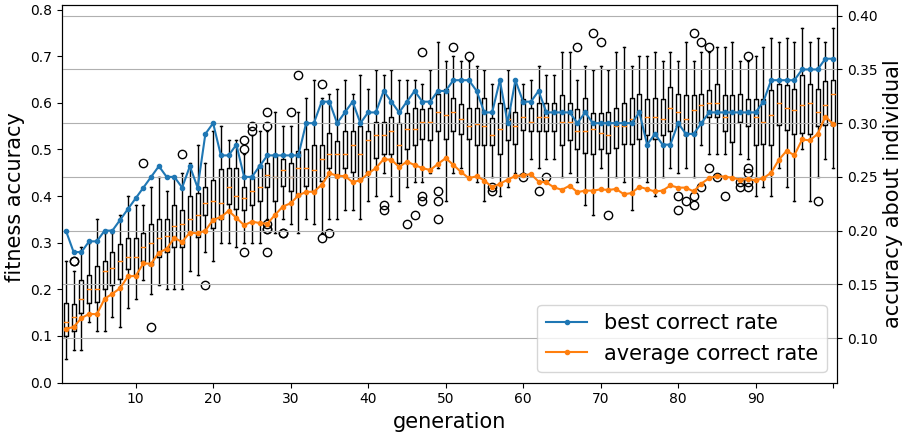
\includegraphics[scale=0.70]{./images/ex2_res_graph.png}
		\caption{実験2 : GA の探索結果\label{fig:ex2_res1}}
	\end{center}
\end{figure}


\begin{figure}[h]
	\begin{center}
		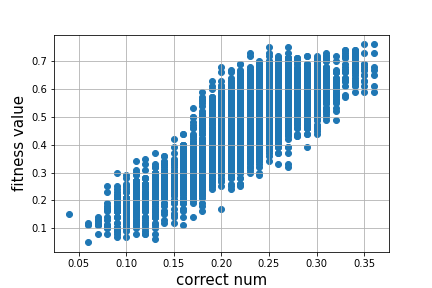
\includegraphics[scale=1.0]{./images/ex2_res_img.png}
		\caption{実験2 : 探索個体の散布図\label{fig:ex2_res2}}
	\end{center}
\end{figure}


次に,表\ref{tb:ex2_res3}に探索された個体によるテスト識別率を示す.
結果は提案手法による疑似ラベルがベースラインおよび
従来の疑似ラベルよりもテスト識別率が劣っていることがわかる.疑似ラベルの精度が低いため
テスト識別率の精度も低くなっていると考えられる.

\begin{table}[h]
	\centering
	\caption{実験2 : テスト識別率\label{tb:ex2_res3}}
	\scalebox{0.8}{
		\begin{tabular}{|c|c|c|} \hline
			$D_{\rm s}$ に対するラベル&テスト識別率&正答率\\ \hline\hline
			正解ラベル&0.822&1.00\\ \hline
			提案手法による疑似ラベル&0.674&0.37\\ \hline\hline
			baseline モデルによる疑似ラベル&0.784&0.74\\ \hline\hline
			baseline (ラベル付きデータのみ)&0.772&$\backslash$\\ \hline
		\end{tabular}
	}
\end{table}

また,実験2では Encoder の学習時間が 1 GPU days かかってはいるものの,
1個体の適応度を出す時間について,実験1に対し16倍ほど速くすることができ,
個体数や世代数を多くするにはベースモデルとして FixMatch よりも SimCLR を用いる方が良いことが分かる.

	\clearpage
	
	\newpage
\changeindent{0cm}
\section{まとめと今後の課題}
\changeindent{2cm}
本研究では,遺伝的アルゴリズムを用いてラベルなしデータに対する疑似ラベル生成手法の提案をした.
また,数値実験から探索された疑似ラベルを用いた学習において精度の低下を確認し,
遺伝的アルゴリズムによるラベル探索は非常に困難であることが分かった.

今後の課題として,遺伝的アルゴリズムのパラメータチューニング及び,
膨大な探索空間に有効に拡張されたアルゴリズムを使用するといった遺伝的アルゴリズムについての改善.また,
validation data についても画像の水増しを行うことや一個体の学習に対するパラメータチューニングといった
適応度計算についての改善の2点が挙げられる.




	\clearpage
	
	\newpage
\changeindent{0cm}
\acknowledgements
\changeindent{2cm}

本研究を進めるにあたりご指導,ご鞭撻を賜りました森直樹教授,岡田真助教授に深く感謝申し上げます.
また,発表スライドや本論文の作成にあたり添削及びアドバイスを下さったソフトウェアシステム研究グループの皆様にも厚く御礼を申し上げ,
感謝の意を表します.
\begin{flushright}
	2021年2月26日
\end{flushright}

	
	% 参考文献
	\clearpage
	%\newpage
\changeindent{0cm}
\begin{thebibliography}{99}
 \changeindent{2cm}
\end{thebibliography}


	\changeindent{0cm}
	%\bibliographystyle{unsrt}
	\bibliographystyle{jabbrvunsrt}
	\bibliography{reference}
	
	
	
\end{document}